\section{Discussion}
The results obtained in Section \ref{results} are summarized in Table \ref{tab:sim_res_worlds} and \ref{tab:sim_res_worlds_active}.
\begin{center}
  \captionof{table}{Simulation results for all environments without active dispersion\label{tab:sim_res_worlds}}
  \begin{tabular}{l|l|l|l|l}
    Environment & 3 agents & 6 agents & 15 agents & 50 agents\\
    \hline
    Tinyworld & 100\% & - & - & - \\ 
    Tinyworld2 & 71.8\% & 98\% & - & - \\
    Rectworld &  22.1\% & 24.5\% & 95\% & - \\
    Complexworld & - & - & - & 15.5\% \\
  \end{tabular}
\end{center}
\begin{center}
  \captionof{table}{Simulation results for all environments with active dispersion\label{tab:sim_res_worlds_active}}
  \begin{tabular}{l|l|l|l|l}
    Environment & 3 agents & 6 agents & 15 agents & 50 agents\\
    \hline
    Tinyworld & 100\% & - & - & - \\ 
    Tinyworld2 & 45.2\% & 100\% & - & - \\
    Rectworld &  25\% & 46\% & 93\% & - \\
    Complexworld & - & - & - & 89\% \\
  \end{tabular}
\end{center}

We start with the most simple environment, Tinyworld, whose simulation results are shown in \ref{tinyworld}. In \figref{fig:3_agnt_tw_k_1_0_distr} and \figref{fig:3_agnt_tw_k_1_1_k_2_1_distr} we clearly see the 
effect of active dispersion. In the case where no active dispersion is used the objective function is constant over the feasible space. Hence the initial configuration is one of 
infinitely many equal valued optima, and Algorithm \ref{alg:alg1} haults after one iteration. In the case where active dispersion is applied the agents spread to the corners of the
feasible space as seen in \figref{fig:3_agnt_tw_k_1_1_k_2_1_distr}. This is due to the fact that $L(\mathbf{X}_{\mathcal{B}_{a}\cup\{a\}})$ is constant over the feasible space, hence the 
local optimization problem \eqref{local_opt_prob} is equivalent to maximizing dispersion between an agent $a$ and its neighbours. In light of \cite{CRB_multilat} the configuration generated
when applying active dispersion in the Tinyworld environment is the superior one, as the convex hull of the agents span a greater area when applying active dispersion than when only maximizing the area covered
by an agent and two of its neighbours. Thus configuration generated by Algorithm \ref{alg:alg1} using active dispersion would allow for more accurate 

The simulations performed for a swarm of size 3 in the Tinyworld2 environment display a weakness of active dispersion. Here the swarm covers a smaller percentage of the 
feasible space when applying active dispersion than when not. This is due to the fact that the dispersion term is weighet to heavily. When the local probability of coverage for an agent is small, i.e. $L(\mathbf{X}_{\mathcal{B}_{a}\cup\{a\}})$ is small 
for all possible values of $\mathbf{x}_{a}$, the value of 
the local objective \eqref{totally_objective} is dominated by the dispersion term. This causes a shift in behaviour. The focus is on dispersion rather than coverage, and Algorithm \ref{alg:alg1} converges
to a solution that gives a smaller percentage of covered area.

For a swarm of 6 agents in the Tinyworld2 environment the case is quite different. Now active dispersion yields a configuration that gives a larger coverage percentage than when no active
dispersion is applied. This result is although not a consequence of clever objective function formulation. As for three agents the active dispersion term dominates the coverage term
in \eqref{totally_objective} due to local probability of coverage being small no matter the value of $\mathbf{x}_{a}$. Hence the agents focus on maximizing dispersion rather than covered area. The 
solution generated by Algorithm \ref{alg:alg1} for 6 agents in the Tinyworld2 environment is identical to the solution generated for 6 agents in the Tinyworld environment when applying active dispersion. 
This makes it obvious that the high percentage of coverage obtained in the Tinyworld2 environment using active dispersion is not caused by the agents meticulously positioning themselves as to maximize the local
probability of coverage. Instead they position themselves so that the maximum dispersion is obtained, and the higher percentage of coverage is simply a lucky bi-effect.

For a swarm of 3 agents in the Rectworld environment, active dispersion does not have a great impact on the percentage of covered area. The final configurations are shown in 
\ref{fig:3_agnt_bw_k_1_0_k_2_1_distr} and \ref{fig:3_agnt_bw_k_1_1_k_2_1_distr}, and it is clear that they do not differ much, except that the configuration obtained when using active dispersion
is translated slightly to the north-east. As shown in \figref{fig:3_agnt_bw_k_1_0_s_traj} and \figref{fig:3_agnt_bw_k_1_1_s_traj} the agents make larger initial steps when active dispersion is applied. This
causes them to move further into the mission space. Thus less of their visual sets are clipped by the walls of the mission space, resulting in a larger percentage of covered area.

Both configurations obtained for 3 agents in the Rectworld environment exhibit the same problematic behaviour. Moving the entire swarm in the north-east direction would yield higher percentage of covered area,
but Algorithm \ref{alg:alg1} converges with the swarm placed so that the area covered by the three agents is clipped by the mission space walls. This is due to Algorithm \ref{alg:alg1} optimizing
the configuration of the swarm one agent at the time. In order to move the entire swarm to the north-east direction, all agents would have to move in the north east direction, and they
would have to do so one at the time. In the configuration shown in \figref{fig:3_agnt_bw_k_1_0_k_2_1_distr} no single agent would increase their local objective by moving, although they would all benefit from each other moving.
Due to no single agent benefiting from moving Algorithm \ref{alg:alg1} converges to a clearly sub-optimal configuration.

In the Rectworld environment we observe for the first time the main benefit of using active dispersion. \figref{fig:6_agnt_bw_k_1_0_k_2_1_distr} shows the configuration obtained
by running Algorithm \ref{alg:alg1} for a swarm of size 6 without active dispersion. Here we see that the three agents in the bottom-left corner stay
at their initial positions throughout the simulation. \figref{fig:bw_x_traj} shows the configuration of the swarm after each iteration of Algorithm \ref{alg:alg1}. It is clear that 
throughout the iterations the visible sets of the bottom three agents are covered by those of the top three agents. Thus the local objective value for the bottom three agents is zero 
throughout the iterations, and any infinitesimal perturbation of their positions cause no change to the objective value, i.e. zero gradient. The SQP solver concludes that the bottom three agents are at a local
optimum, and no change is made to their position. The configuration generated for a swarm of size 6 using active dispersion does not exhibit the same behaviour as the afforementioned configuration. Yet again this can be attributed to the
larger initial step sizes due to active dispersion (see \ref{fig:6_agnt_bw_k_1_0_s_traj} and \ref{fig:6_agnt_bw_k_1_1_s_traj}) causing no agents to have their entire visible set covered by those of three or more other agents.
\begin{figure}[H]
  \centering
  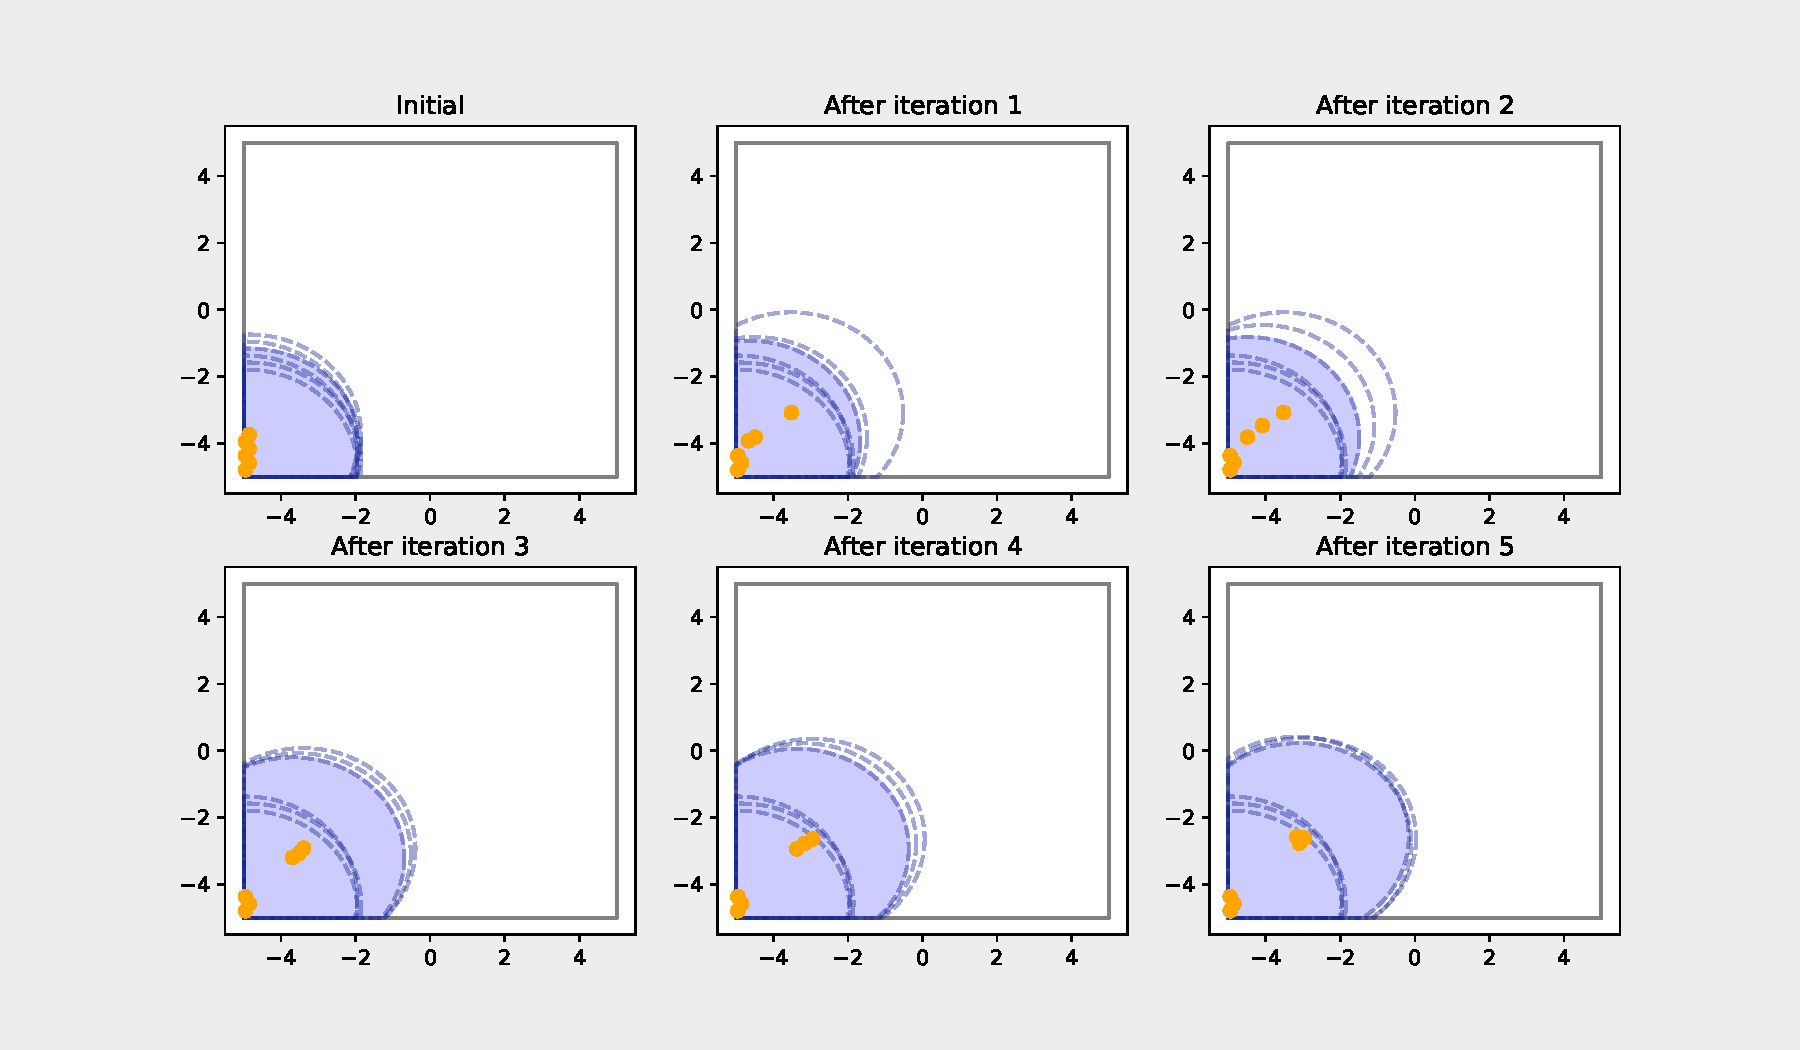
\includegraphics[width=\textwidth]{figs/bigworld_6_agnt_k_1_0_k_2_1_x_traj.pdf}
  \caption{Intermediate configurations for 6 agents in the Rectworld environment with $k_{1} = 0$ (no active dispersion).}
  \label{fig:bw_x_traj}
\end{figure}



From the simulations in the Rectworld environment with 6 agents and the Complexworld environment it is 
clear that active dispersion prevents convergence to clearly sub-optimal local maxima. As seen in \figref{fig:6_agnt_bw_k_1_0_k_2_1_distr} three of the 
6 agents do not move whatsoever from their initial configuration. This is due to the fact that once the three first agents have performed one optimization and moved to the 
optimum, the three remaining agents cover a small area in the lower left hand corner of the feasible space. When optimizing the position of each of the remaining three agents
one at the time, moving will only decrease their local objective. This results on none of the remaining agents moving. Thus once the three agents that have moved converge (after eight iterations as seen in \figref{fig:6_agnt_bw_k_1_0_s_traj}) Algorithm \ref{alg:alg1} haults and the resulting configuration 
can be seen in the rightmost plot in \figref{fig:6_agnt_bw_k_1_0_k_2_1_distr}. This configuration is clearly not an optimal solution as translating all agents in the north-east direction would yield a higher 
percentage of covered area. 


Seen as the objective when no active dispersion is applied is the area covered
by an agent and excatly two of its neighbours, the remaining three agents lie at a local optimum after the initial three agents have moved.